\documentclass[12pt]{beamer}
\usepackage{graphicx}
\usefonttheme[onlymath]{serif}
\usepackage{amsmath}
\renewcommand{\vec}[1]{\mathbf{#1}}
\newcommand{\grad}{\nabla}
\newcommand{\partiald}[2]{\frac{\partial {#1} }{\partial {#2}}}
\usepackage[english]{babel}
\usepackage[utf8x]{inputenc}
\usepackage{amsmath,amsfonts,amsthm,graphicx}
\usepackage{bm,amsmath,bbm,amsfonts,nicefrac,latexsym,amsmath,amsfonts,amsbsy,amscd,amsxtra,amsgen,amsopn,bbm,amsthm,amssymb,textcomp,graphicx,float,verbatim,physics,hyperref,tabu, marvosym}


%Information to be included in the title page:
\usepackage{bm}%fette Symbole(Vektoren)
\usepackage{nicefrac}
\usepackage{xcolor}
\usepackage{import}


\newcommand\Ccancel[2][black]{\renewcommand\CancelColor{\color{#1}}\xcancel{#2}}

\newcommand*{\HomePath}{} %Set Home Path

\graphicspath {{\HomePath Plots/}{Plots/}} %Set Plot Path
\subimport{}{commands.tex} %Import commands




\mode<presentation>
{
	\usetheme{Madrid}     
	\usecolortheme{}
	\usefonttheme{default}  
	\setbeamertemplate{navigation symbols}{}
	\setbeamertemplate{caption}[numbered]
	\setbeamercolor{block title}{bg=orange!70}
	
} 

\usepackage[english]{babel}
\usepackage[utf8x]{inputenc}


\title[Rossby Waves]{Rossby Waves}
\author{Manu Sidhu, Sam Harrison, Philipp Breul, Edward Calver, Cathie Wells}
\institute{University of Reading and Imperial College London}
\begin{document}
	
	\begin{frame}
	\titlepage
\end{frame}

\begin{frame}{Overview}

\begin{itemize}
	\item Introduce Rossby waves and the Shallow Water Equations (SWE). (Manu)
	\item Potential Vorticity. (Philipp)
	\item Linearisation. (Sam)
	\item (Edward)
	\item Application of Rossby Waves. (Cathie)
\end{itemize}

\begin{figure}[H]
	\centering
	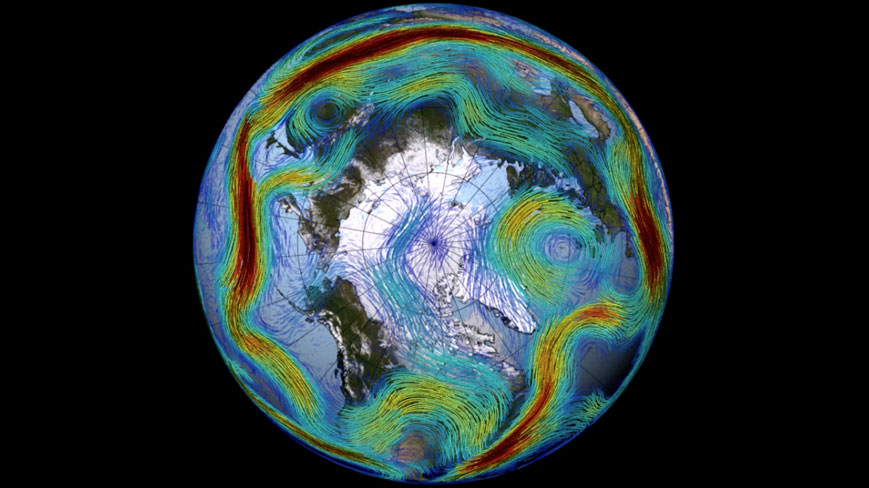
\includegraphics[width=0.5\linewidth]{Rossby_Wave.jpg}
\end{figure}   

\end{frame}


\begin{frame}{Introduction - Rossby Waves}

\begin{itemize}
\item Identified by Carl-Gustad Arvid Rossby.
\item Large meanders in high altitude winds.
\item Responsible for the weather at mid latitudes.
\item Caused by the Earth's rotation.
\item Two types of Rossby wave
\end{itemize}

\begin{table}[H]
\begin{center}
	\begin{tabular}{ |c|c|} 
		\hline
		\textbf{Barotropic} & \textbf{Baroclinic} \\
		\hline 
		Free wave & Forced wave \\  
		Progress eastward and fast moving & Slow moving ($cm/s$) \\
		Free travelling & Quasi stationary \\
		No significant vertical changes & Vertical changes \\
		\hline
	\end{tabular}
\end{center}
\end{table}

\begin{itemize}
\item Caused by conservation of \textbf{potential vorticity}.
\end{itemize}

\end{frame}

\begin{frame}{How do we get to the Rossby Waves?}

\begin{itemize}
\item Navier-Stokes \MVRightarrow  Shallow Water Equations (SWE) \MVRightarrow  Rossby Waves
\end{itemize}

\vspace{15pt}


The shallow water equation -
\begin{equation}
\frac{\partial{\textbf{u}}}{\partial{t}} + \textbf{u}.\nabla\textbf{u} + f \textbf{z} \times \textbf{u} = -g \nabla h
\end{equation}

The shallow water mass conservation - 

\begin{equation}
\frac{Dh}{Dt} + (h\nabla \textbf{u}) = 0.
\end{equation}
\end{frame}
\begin{frame}{What are the Shallow Water Equations?}

\begin{itemize}
\item A set of hyperbolic PDEs governing fluid flow in the oceans, coastal regions, rivers and channels.
\item Consider the vertical length scale to be significantly smaller than the horizontal length scale.
\item The SWE are derived from the Navier-Stokes equations.
\item The Navier-Stokes equations are themselves derived from the equations for conservation of momentum (1) and the conservation of mass (2).
\end{itemize}

\vspace{-15pt}

\begin{equation}   
\rho(\frac{\partial{\textbf{u}}}{\partial{t}} + \textbf{u}.\nabla \textbf{u}) = -\nabla p  + \mu \nabla^2\textbf{u} + \rho \textbf{g},
\end{equation}

where $u=$ velocity, $p=$ pressure, $\rho=$ density and $\mu=$ viscosity.

\begin{equation}
\frac{\partial{\rho}}{\partial{t}} + (\nabla.\rho \textbf{u}) = 0.
\end{equation}

\end{frame}


\begin{frame}{Deriving the Shallow Water Equations}

\begin{itemize}
\item Derive the Navier-Stokes equations from the conservation laws (1) and (2).
\item Specify boundary conditions for the Navier-Stokes equations for a water column.
\item Use the boundary conditions to depth integrate the Navier-Stokes equations.
\end{itemize}

The Shallow Water Equation -
\begin{equation}
\frac{\partial{\textbf{u}}}{\partial{t}} + \textbf{u}.\nabla\textbf{u} + f \textbf{z} \times \textbf{u} = -g \nabla h
\end{equation}

\begin{itemize}
\item Linearise the system of equations to perform analysis on.
\end{itemize}

\end{frame}
\begin{frame}
\frametitle{Vorticity Equation}
Rewrite  shallow water equations in terms of \textit{relative vorticity} $\zeta$
\vspace{0.5cm}
\begin{itemize}
	\item take the curl $\nabla \times \left(...\right)$
	\item $\pder{\zeta}{t}+\bm{u}\nabla(\zeta+f)=(\zeta+f)\nabla \bm{u}$
\end{itemize}
\vspace{0.5cm}
Inserting the mass conservation $\mder{h}{t}+h\nabla\bm{u}=0$, we can restate the equations as 
\vspace{0.5cm}
\begin{itemize}
	\item $\mder{}{t}\left(\frac{\zeta+f}{h}\right)=0$
\end{itemize}
\vspace{0.5cm}
We found a conserved quantity! It is called \textbf{potential vorticity}. 
\end{frame}


\begin{frame}
\frametitle{Potential Vorticity}
What is potential vorticity $q=\frac{\zeta+f}{h}, \mder{}{t}q=0$?
\vspace{0.5cm}
\begin{itemize}
\item Continuum equivalent of \textit{angular momentum} conservation
\end{itemize}
\vspace{0.5cm}
In $f$-plane approximation, $f=f_0=$const. :
\vspace{0.2cm}
\begin{columns}
\begin{column}{0.48\textwidth}
	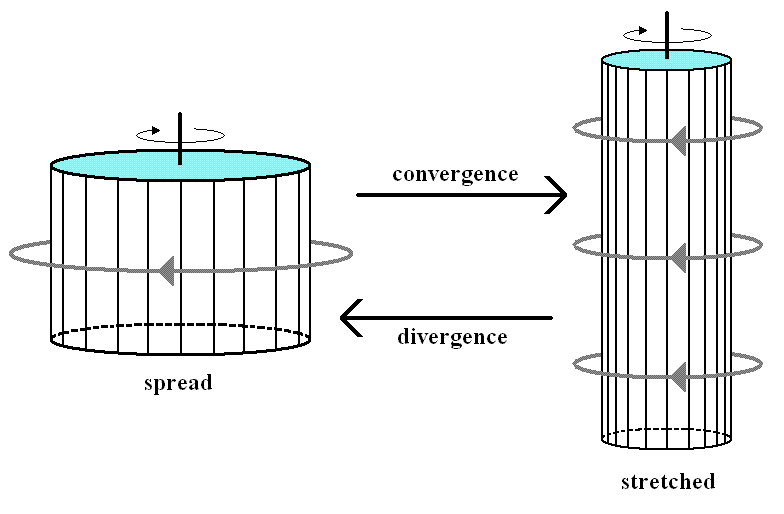
\includegraphics[width=\linewidth]{Potential_vorticity_conservation}
\end{column}
\begin{column}{0.48\textwidth}
	\begin{itemize}
		\item Change in $\zeta$ has to be compensated by change in hight $h$
	\end{itemize}
\end{column}
\end{columns}
\end{frame}


\begin{frame}
\frametitle{Potential Vorticity}
In $\beta$-plane approximation $f=f_0+\beta y$ is not constant. \hfill $\color{blue}\boxed{q=\frac{\zeta+f}{h}}$\\
\vspace{0.5cm}
Fluid parcels can move north-/southward when changing vorticity $\zeta$.
\begin{columns}
\begin{column}{0.55\textwidth}
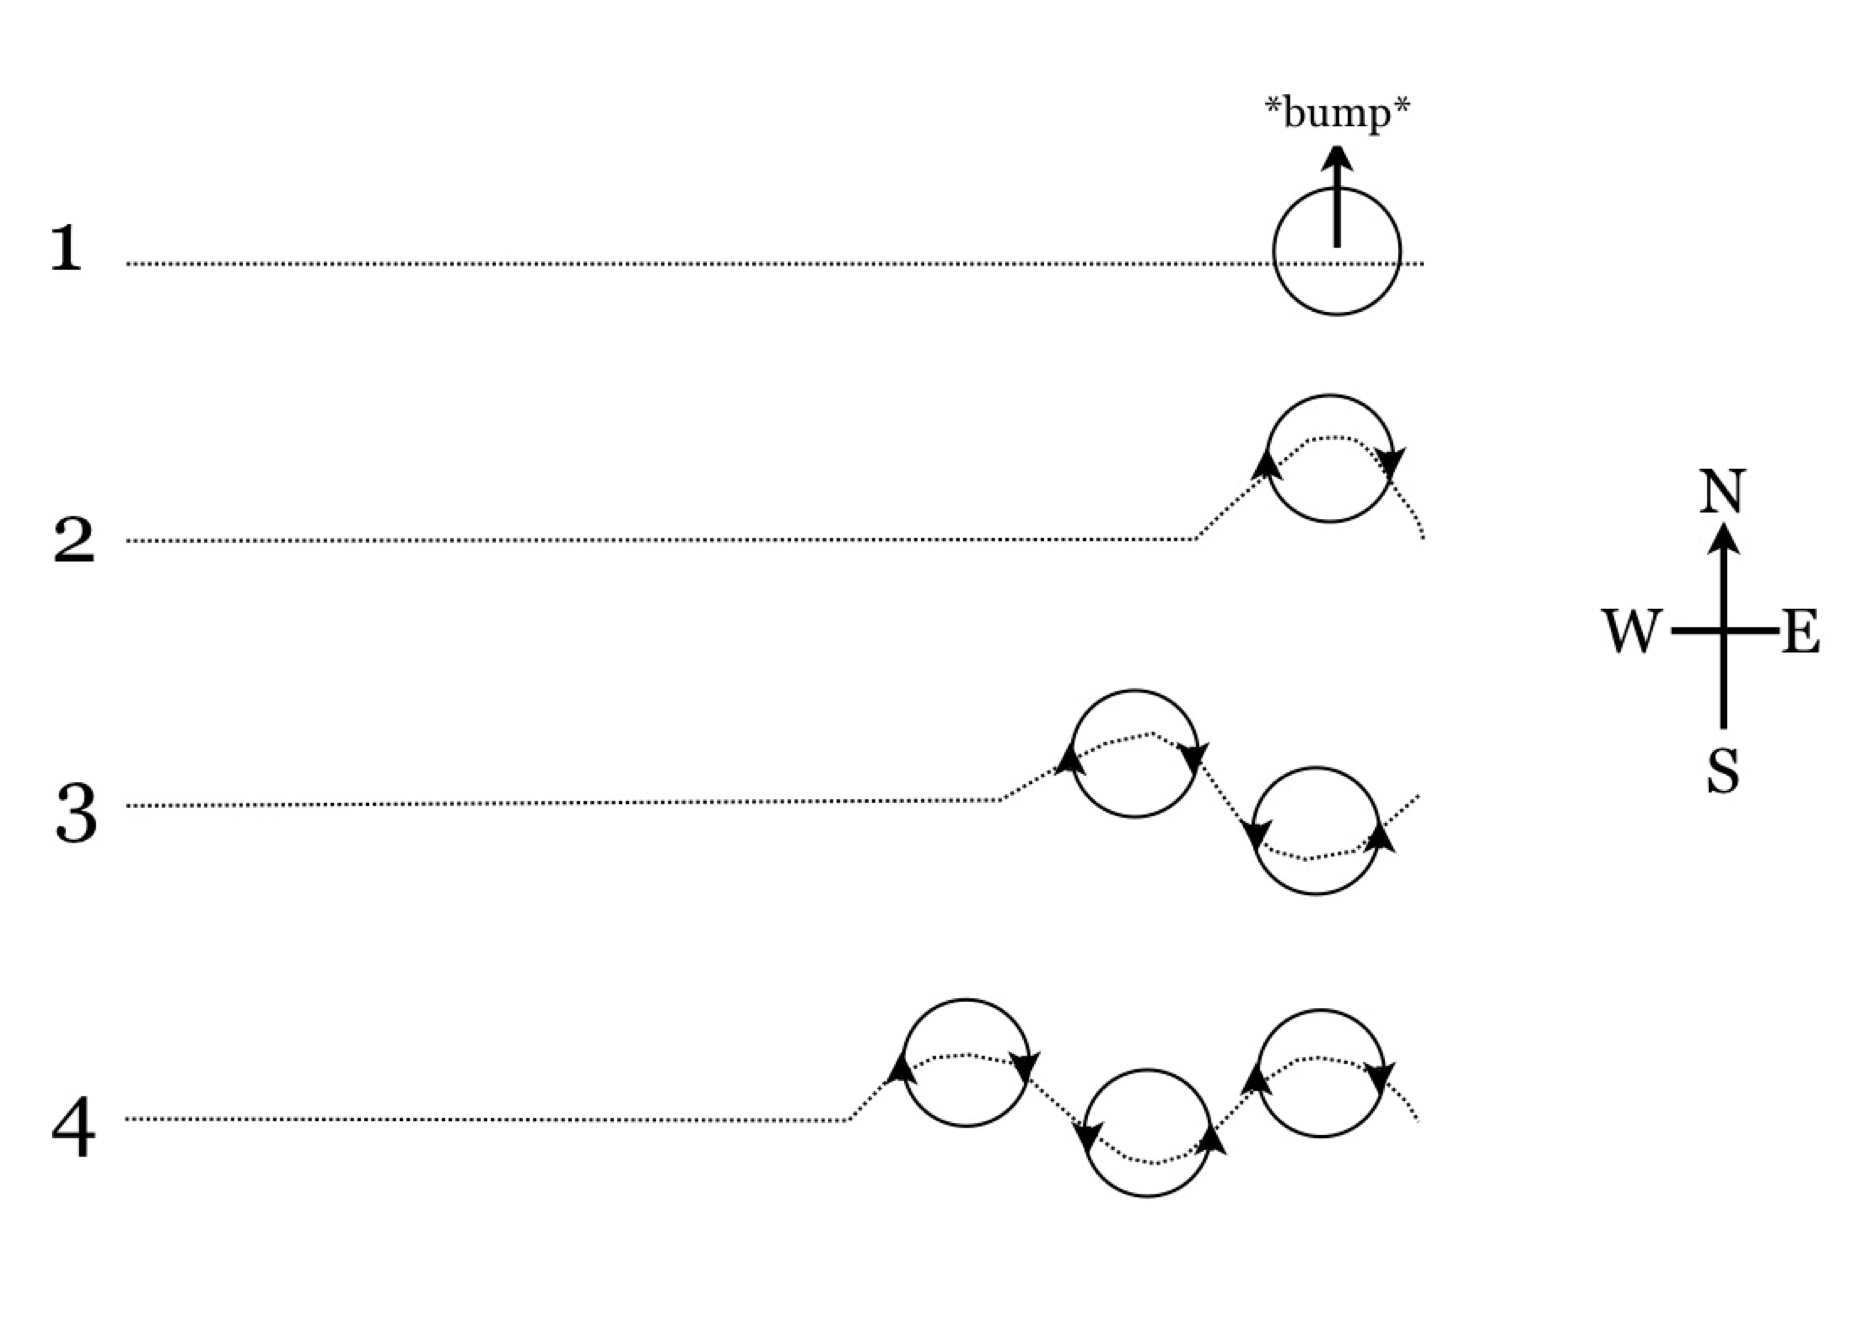
\includegraphics[width=\linewidth]{beta_plane}
\end{column}
\begin{column}{0.45\textwidth}
\begin{itemize}
	\item Additionally induce movement on neighboured fluid particles
\end{itemize}
\end{column}
\end{columns}
\end{frame}
% TODO INSERT EDWARD's HERE 
\begin{frame}
\frametitle{Quasi stationary synoptic Rossby waves high amplitude during weather events }
\framesubtitle{by Petoukhov, Rahmstorf, Pteri and Schellnhuber 2013}
\begin{itemize}
	\item Investigated physical model of quasi resonance effect.
	\item Forced wave trapping a free wave.
	\item Amplification of pressure system.
	\item Extreme weather results.
\end{itemize}
\centering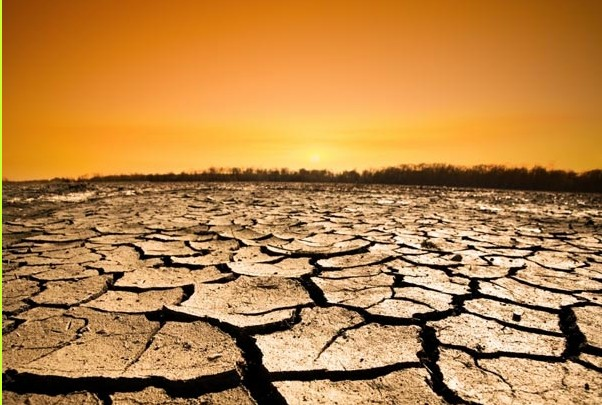
\includegraphics[height=0.4\textheight]{drought}

\end{frame}
\begin{frame}
\frametitle{Amplified mid-latitude planetary waves favour particular regional weather extremes}
\framesubtitle{ 
by Screen and Simmonds }
\begin{itemize}
\item Looked at distribution of quasi resonance events.
\item Examined links between temperature and precipitation anomalies and abnormal quasi stationary wave amplitude from 1979 to 2012.

\end{itemize}
\centering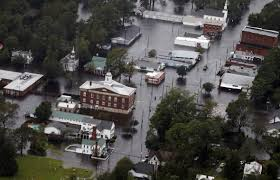
\includegraphics[height=0.4\textheight]{flood}
\end{frame}

\begin{frame}
\frametitle{40 most extreme temperature and precipitation events in the mid latitudes between 1979 and 2012.}
\centering
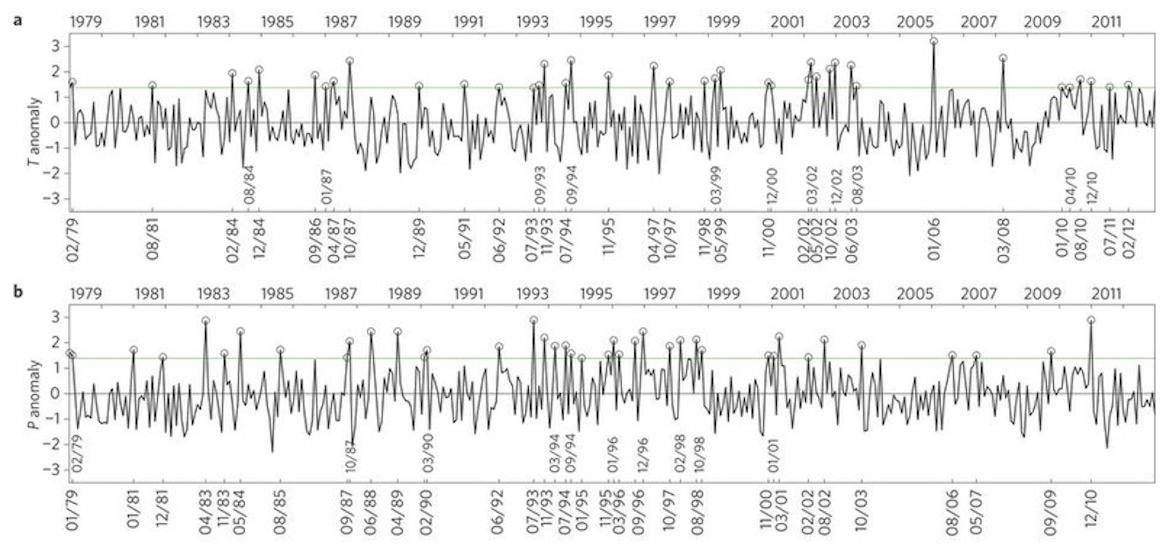
\includegraphics[scale=0.53]{Cathie1}


\end{frame}
\begin{frame}
\frametitle{Anomalies: Prolonged periods over a large area}
\begin{tabular}{c c}
\Large{Temperature}&\vspace{5pt}\\

\large{Positive: abnormally high}	&	\large{Negative: abnormally low}\vspace{20pt}\\

\Large{Precipitation}&\vspace{5pt}\\
\large{Positive: abnormally wet} &		\large{Negative: abnormally dry}\\
\end{tabular}
\end{frame}
\begin{frame}
\frametitle{Mid latitude regions of the Northern hemisphere examined}
\centering
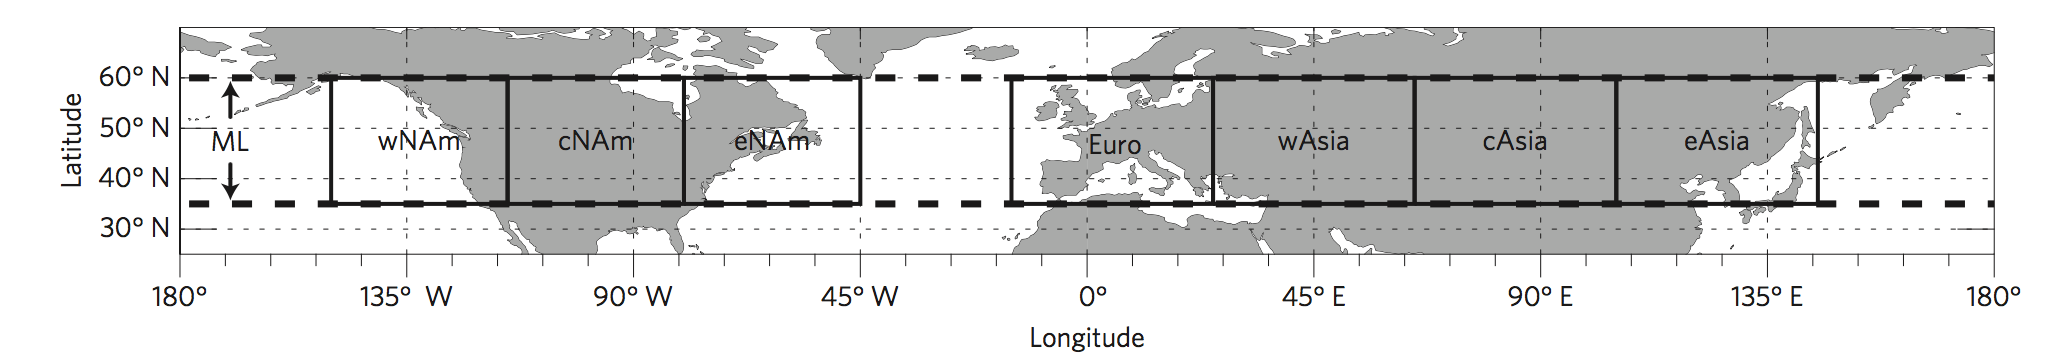
\includegraphics[scale=0.3]{Cathie2}
\end{frame}
\begin{frame}
\frametitle{Charts to show the normalized amplitude anomalies for each extreme temperature event, in order of severity of weather, taking the most extreme events on the left.}
\centering
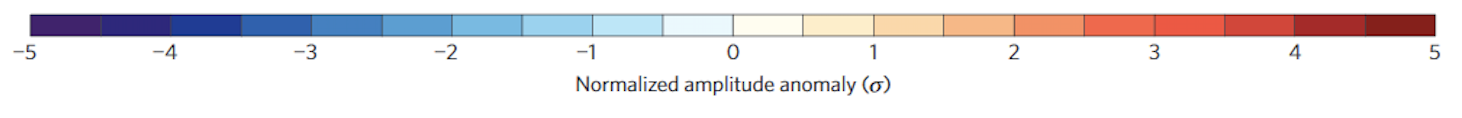
\includegraphics[scale=0.4]{Cathie4}
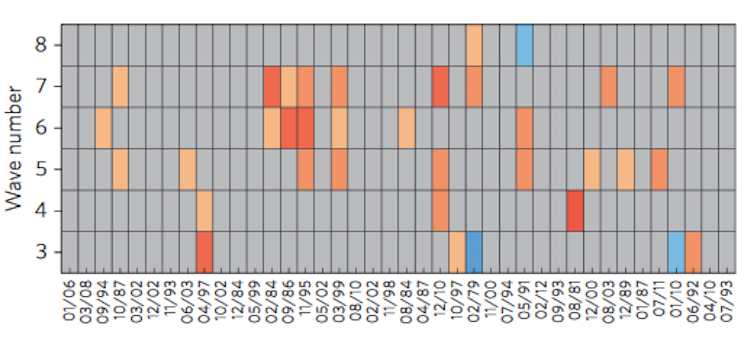
\includegraphics[scale=0.7]{Cathie5}
\end{frame}
\begin{frame}
\frametitle{Charts to show the normalized amplitude anomalies for each extreme precipitation event, in order of severity of weather, taking the most extreme events on the left.}
\centering
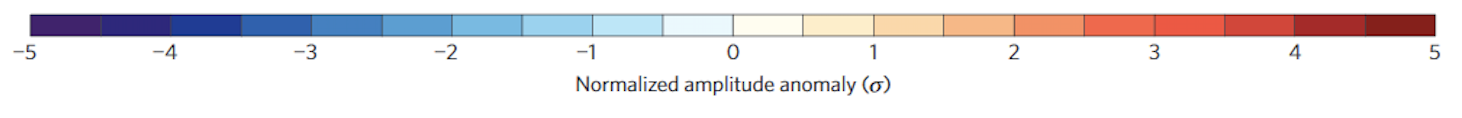
\includegraphics[scale=0.4]{Cathie4}
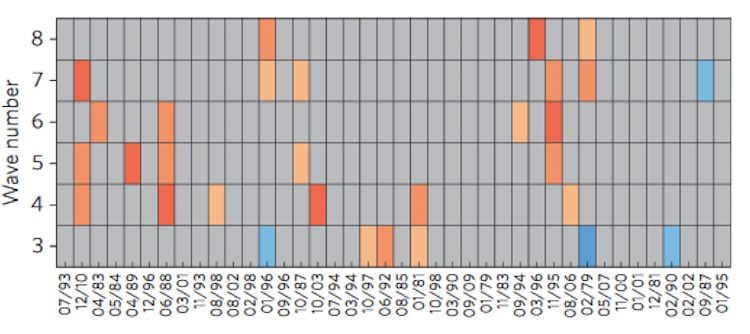
\includegraphics[scale=0.7]{Cathie6}
\end{frame}
\begin{frame}
\frametitle{Distributions comparing observed frequency of anomalous amplitudes of baroclinic Rossby waves during periods of extreme weather and the distributions expected from climatology across each examined region.}
\centering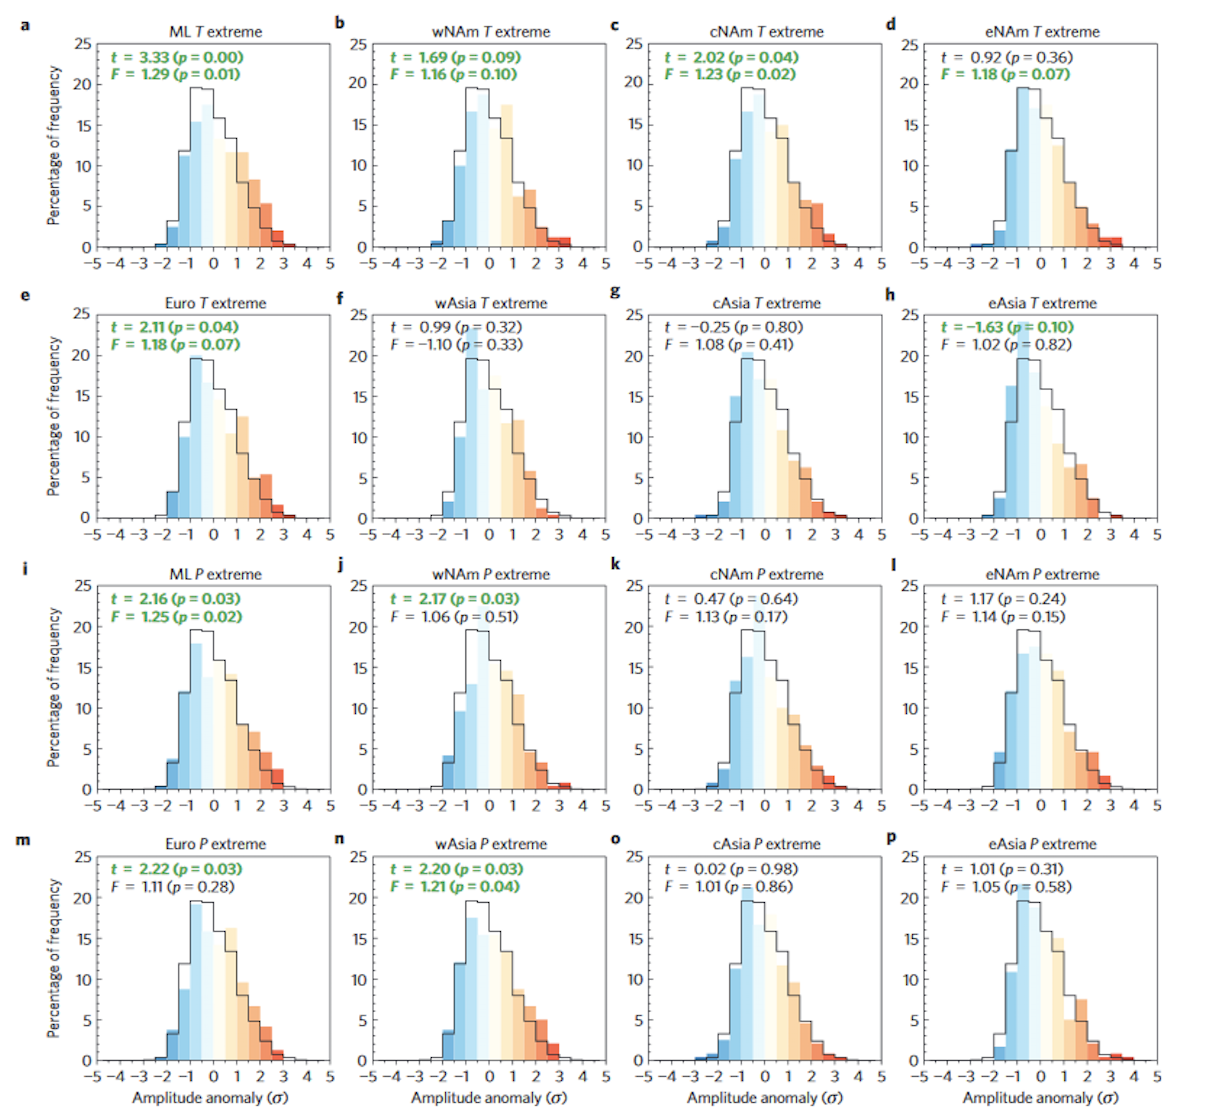
\includegraphics[scale=0.3]{Cathie7}
\end{frame}
\begin{frame}
\frametitle{Future Forecast}
\centering
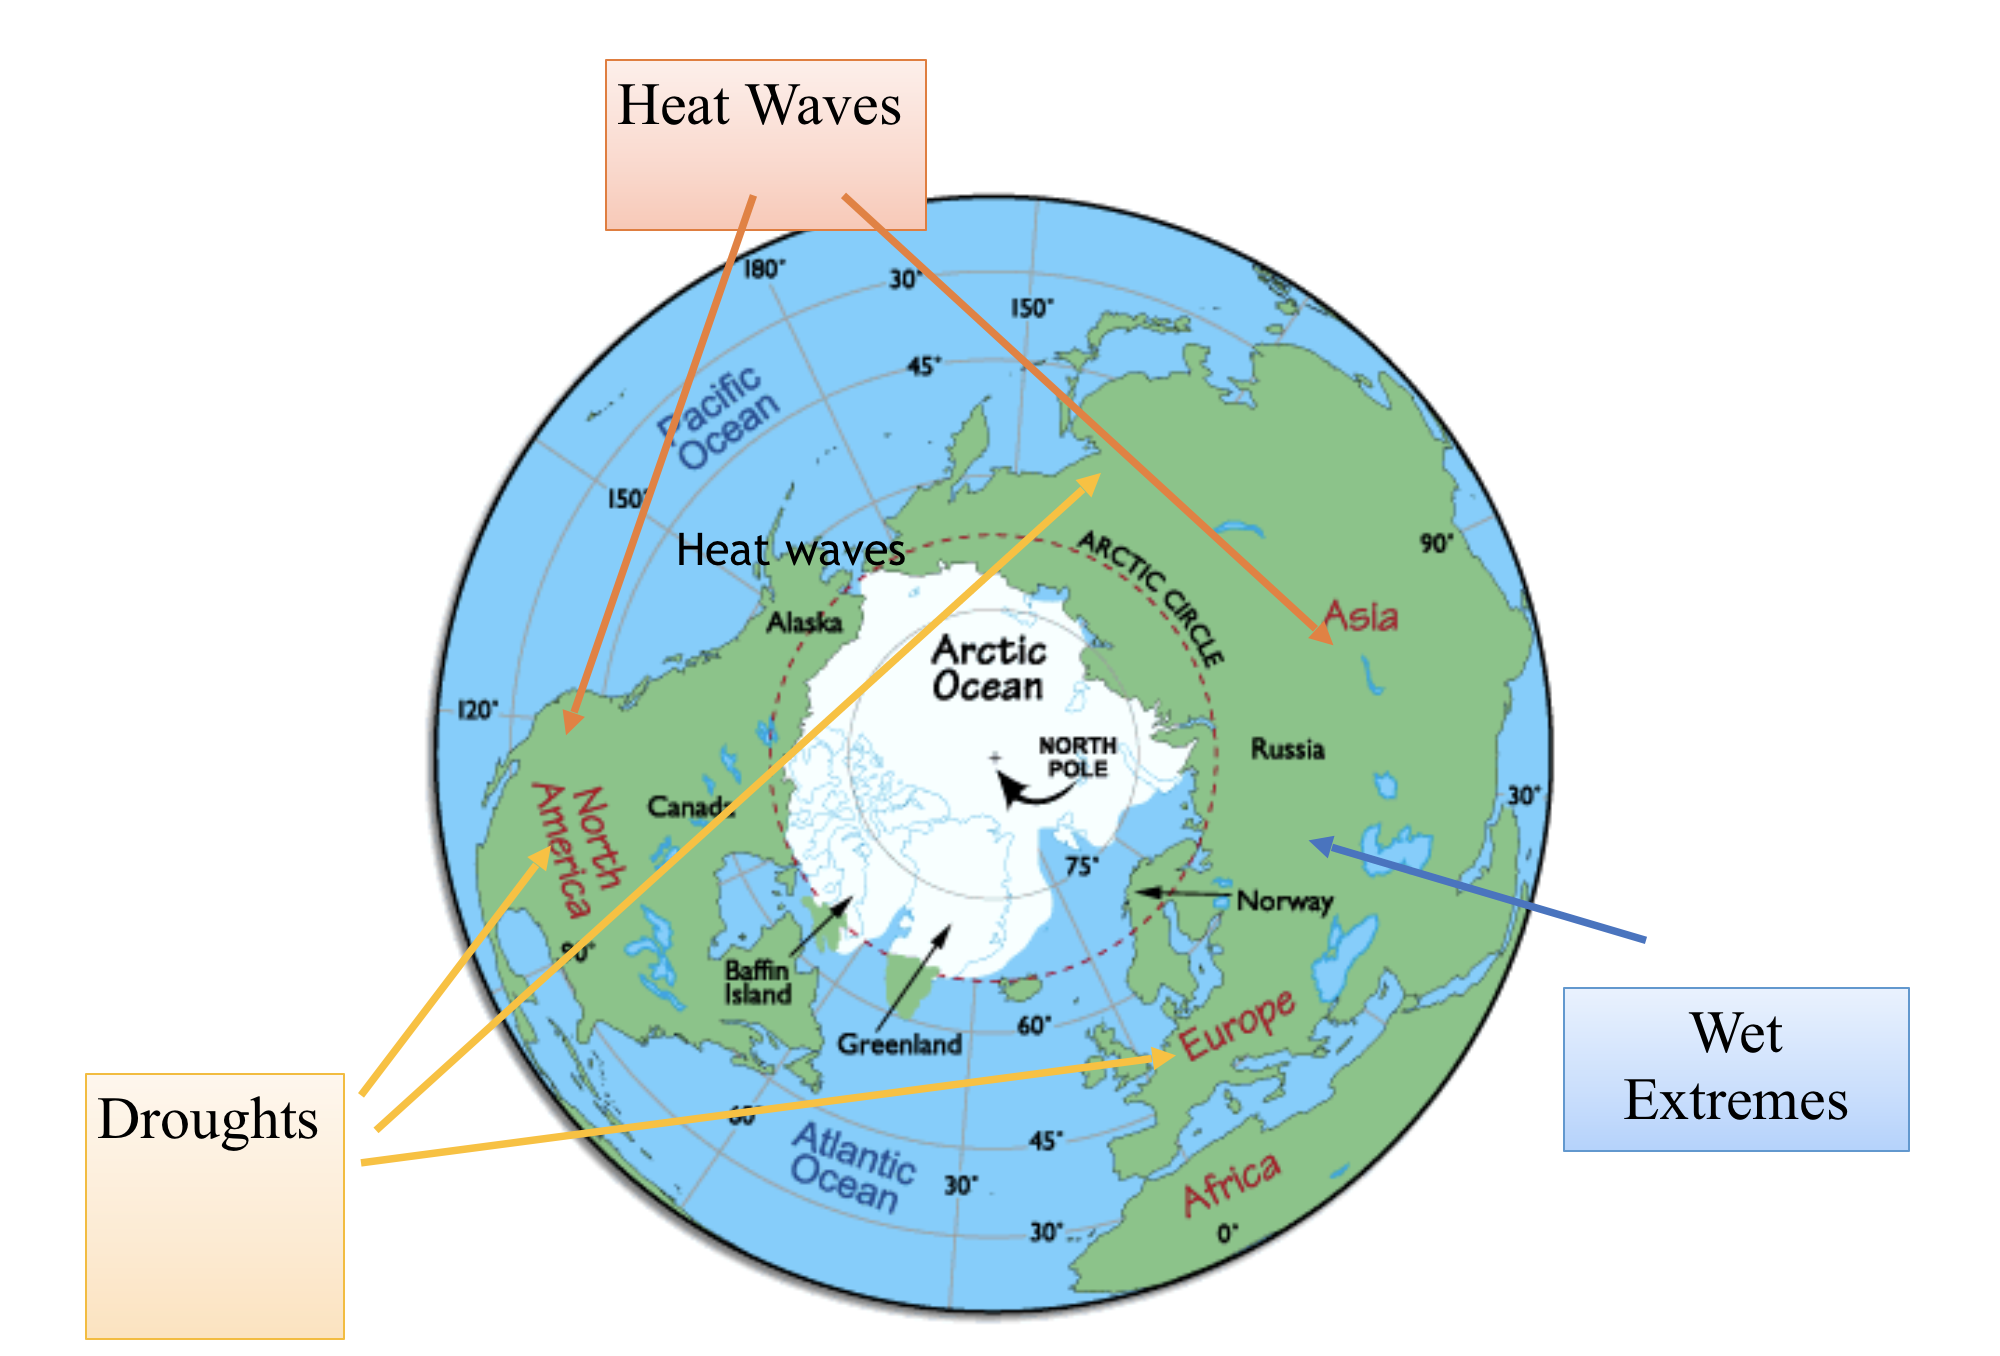
\includegraphics[scale=0.3]{Cathie8}


\end{frame}
\end{document}